% Options for packages loaded elsewhere
\PassOptionsToPackage{unicode}{hyperref}
\PassOptionsToPackage{hyphens}{url}
%
\documentclass[
]{book}
\usepackage{amsmath,amssymb}
\usepackage{iftex}
\ifPDFTeX
  \usepackage[T1]{fontenc}
  \usepackage[utf8]{inputenc}
  \usepackage{textcomp} % provide euro and other symbols
\else % if luatex or xetex
  \usepackage{unicode-math} % this also loads fontspec
  \defaultfontfeatures{Scale=MatchLowercase}
  \defaultfontfeatures[\rmfamily]{Ligatures=TeX,Scale=1}
\fi
\usepackage{lmodern}
\ifPDFTeX\else
  % xetex/luatex font selection
\fi
% Use upquote if available, for straight quotes in verbatim environments
\IfFileExists{upquote.sty}{\usepackage{upquote}}{}
\IfFileExists{microtype.sty}{% use microtype if available
  \usepackage[]{microtype}
  \UseMicrotypeSet[protrusion]{basicmath} % disable protrusion for tt fonts
}{}
\makeatletter
\@ifundefined{KOMAClassName}{% if non-KOMA class
  \IfFileExists{parskip.sty}{%
    \usepackage{parskip}
  }{% else
    \setlength{\parindent}{0pt}
    \setlength{\parskip}{6pt plus 2pt minus 1pt}}
}{% if KOMA class
  \KOMAoptions{parskip=half}}
\makeatother
\usepackage{xcolor}
\usepackage{longtable,booktabs,array}
\usepackage{calc} % for calculating minipage widths
% Correct order of tables after \paragraph or \subparagraph
\usepackage{etoolbox}
\makeatletter
\patchcmd\longtable{\par}{\if@noskipsec\mbox{}\fi\par}{}{}
\makeatother
% Allow footnotes in longtable head/foot
\IfFileExists{footnotehyper.sty}{\usepackage{footnotehyper}}{\usepackage{footnote}}
\makesavenoteenv{longtable}
\usepackage{graphicx}
\makeatletter
\def\maxwidth{\ifdim\Gin@nat@width>\linewidth\linewidth\else\Gin@nat@width\fi}
\def\maxheight{\ifdim\Gin@nat@height>\textheight\textheight\else\Gin@nat@height\fi}
\makeatother
% Scale images if necessary, so that they will not overflow the page
% margins by default, and it is still possible to overwrite the defaults
% using explicit options in \includegraphics[width, height, ...]{}
\setkeys{Gin}{width=\maxwidth,height=\maxheight,keepaspectratio}
% Set default figure placement to htbp
\makeatletter
\def\fps@figure{htbp}
\makeatother
\setlength{\emergencystretch}{3em} % prevent overfull lines
\providecommand{\tightlist}{%
  \setlength{\itemsep}{0pt}\setlength{\parskip}{0pt}}
\setcounter{secnumdepth}{5}
\usepackage{booktabs}
\usepackage{booktabs}
\usepackage{longtable}
\usepackage{array}
\usepackage{multirow}
\usepackage{wrapfig}
\usepackage{float}
\usepackage{colortbl}
\usepackage{pdflscape}
\usepackage{tabu}
\usepackage{threeparttable}
\usepackage{threeparttablex}
\usepackage[normalem]{ulem}
\usepackage{makecell}
\usepackage{xcolor}
\ifLuaTeX
  \usepackage{selnolig}  % disable illegal ligatures
\fi
\usepackage[]{natbib}
\bibliographystyle{plainnat}
\IfFileExists{bookmark.sty}{\usepackage{bookmark}}{\usepackage{hyperref}}
\IfFileExists{xurl.sty}{\usepackage{xurl}}{} % add URL line breaks if available
\urlstyle{same}
\hypersetup{
  pdftitle={Streetlight and Transport Walking},
  pdfauthor={Tharindu Bandara},
  hidelinks,
  pdfcreator={LaTeX via pandoc}}

\title{Streetlight and Transport Walking}
\author{Tharindu Bandara}
\date{2024-04-06}

\begin{document}
\maketitle

{
\setcounter{tocdepth}{1}
\tableofcontents
}
\hypertarget{data-preparation}{%
\chapter{Data preparation}\label{data-preparation}}

The same steps followed as Gavin did for his 2014 paper (chapter 3).

\begin{itemize}
\tightlist
\item
  Excluded the participants who moved residence in between surveys
\item
  Excluded the respondents who were not the same person at each wave
\item
  Excluded the respondents who had missing values for transport walking for all waves
\item
  Excluded the participants who had missing values for education
\end{itemize}

\hypertarget{streetlight-count}{%
\chapter{Streetlight count}\label{streetlight-count}}

Streetlights is the built environment attribute of interest.

\begin{itemize}
\tightlist
\item
  Street light BE attribute is measured as 1km network buffer of residence.
\end{itemize}

\hypertarget{descriptives}{%
\section{Descriptives}\label{descriptives}}

\hypertarget{descriptive-statistics-of-streetlight-counts-at-each-wave.}{%
\subsection{Descriptive statistics of Streetlight counts at each wave.}\label{descriptive-statistics-of-streetlight-counts-at-each-wave.}}

--\textgreater{}

\hypertarget{distribution}{%
\subsection{Distribution}\label{distribution}}

--\textgreater{}

--\textgreater{}

\hypertarget{one-way-anova-tests}{%
\section{One-way ANOVA tests}\label{one-way-anova-tests}}

--\textgreater{}

--\textgreater{}

--\textgreater{}

--\textgreater{}

\hypertarget{sample-profile}{%
\chapter{Sample Profile}\label{sample-profile}}

Never walker is defined as participants who reportedly didn't walk for transport at each wave they responded to.

--\textgreater{}

\hypertarget{cross-sectional-analysis}{%
\chapter{Cross Sectional Analysis}\label{cross-sectional-analysis}}

Excluded movers (n = 1916 participants), as most of them do not have streetlight counts after the 1st wave. Therefore, streetlight count measured at wave 1 used for this cross-sectional analysis at each wave.

Transport walking:

\begin{itemize}
\tightlist
\item
  Walked or not (logistic regression)
\item
  Minutes of walking (linear regression, only with walkers)
\end{itemize}

BE attribute:

\begin{itemize}
\tightlist
\item
  Baseline streetlight counts
\end{itemize}

Adjusted for:

\begin{itemize}
\tightlist
\item
  Sex
\item
  Baseline age
\item
  Baseline education level (categorical)
\item
  Baseline occupation level (categorical)
\item
  Baseline income level (categorical)
\item
  Baseline neighbourhood disadvantage quintiles (categorical)
\end{itemize}

--\textgreater{}

\hypertarget{longitudinal-analysis}{%
\chapter{Longitudinal Analysis}\label{longitudinal-analysis}}

--\textgreater{}

\hypertarget{plots}{%
\section{Plots}\label{plots}}

\hypertarget{proportion-of-transport-walkers-vs-streetlight-count-by-sex}{%
\subsection{Proportion of transport walkers Vs streetlight count by sex}\label{proportion-of-transport-walkers-vs-streetlight-count-by-sex}}

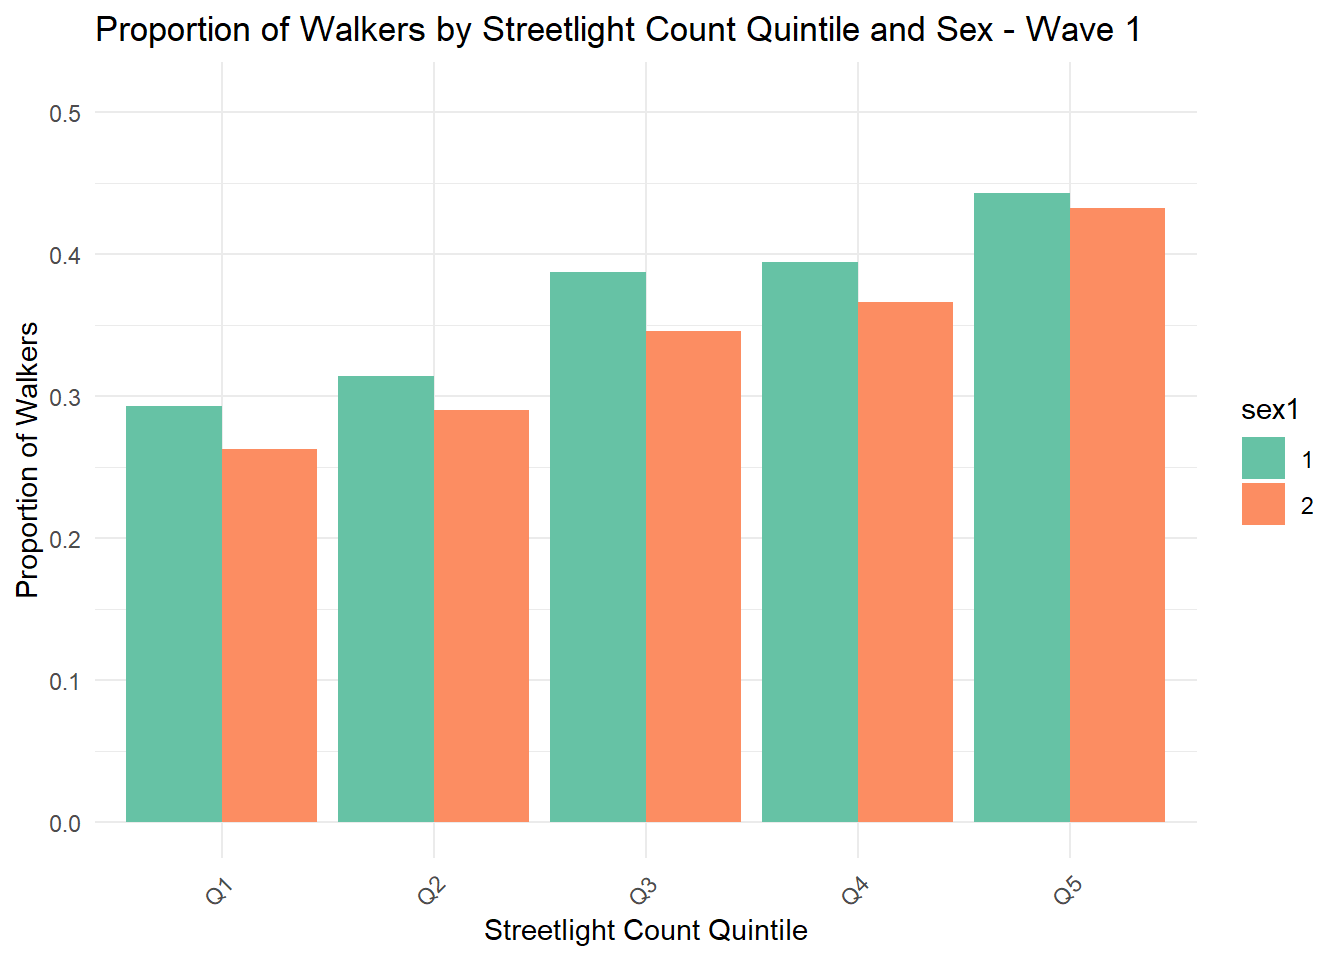
\includegraphics{_main_files/figure-latex/walkers.Prop_vs_SL_plot-1.pdf} 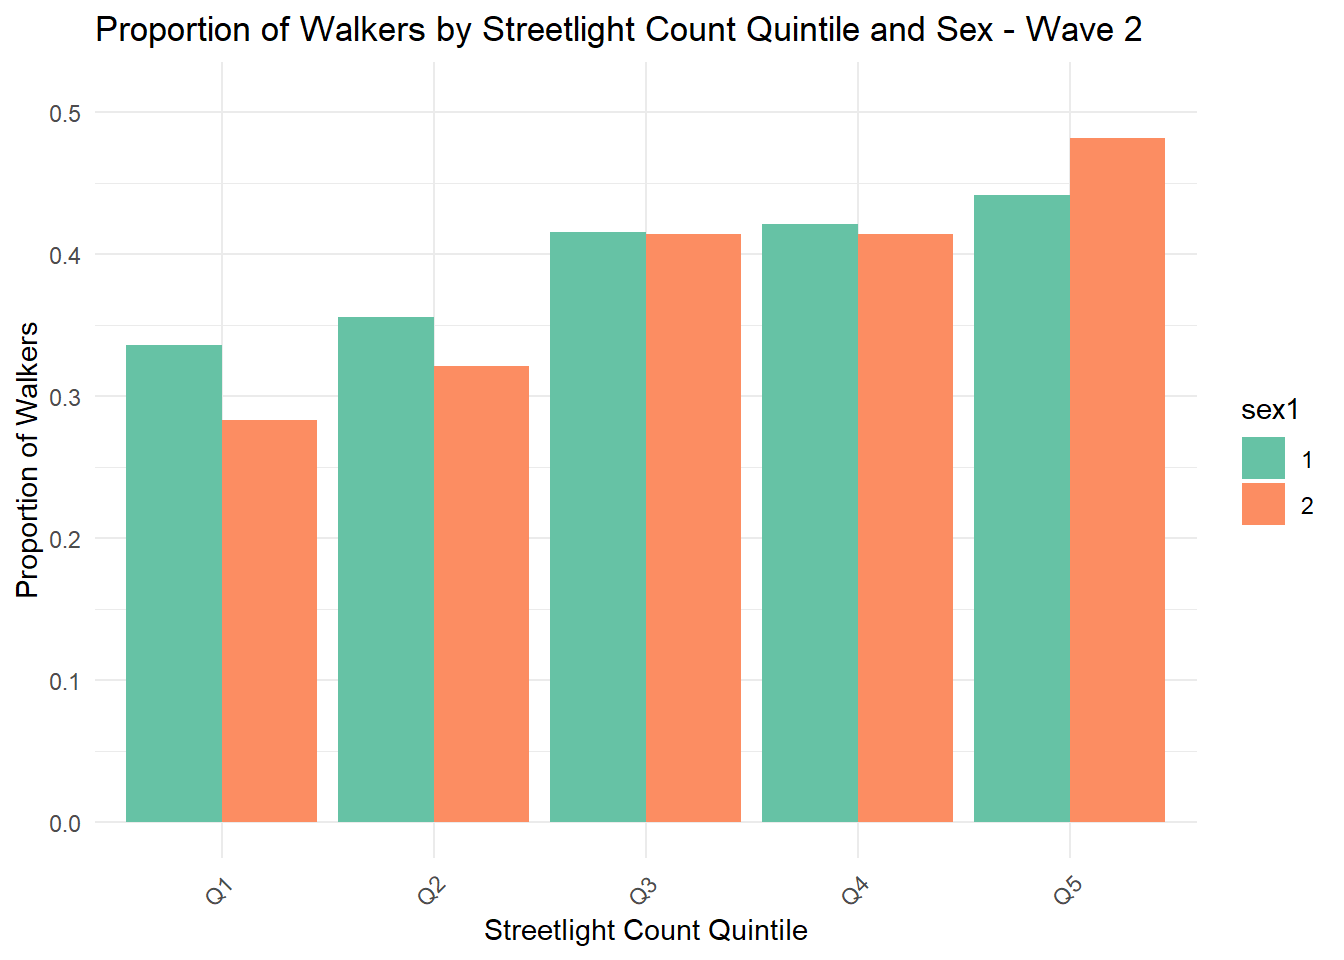
\includegraphics{_main_files/figure-latex/walkers.Prop_vs_SL_plot-2.pdf} 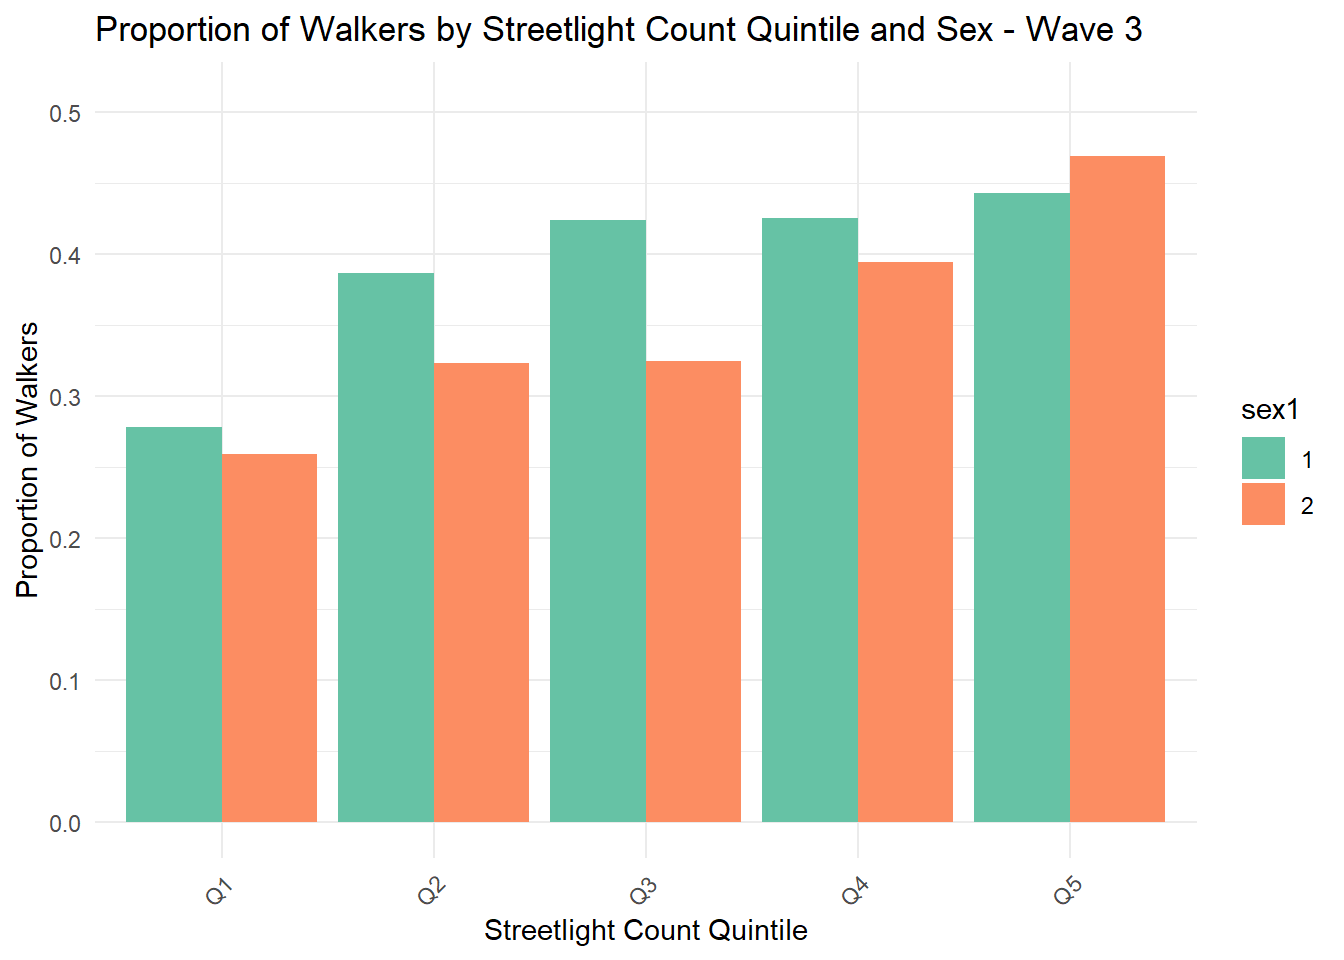
\includegraphics{_main_files/figure-latex/walkers.Prop_vs_SL_plot-3.pdf} 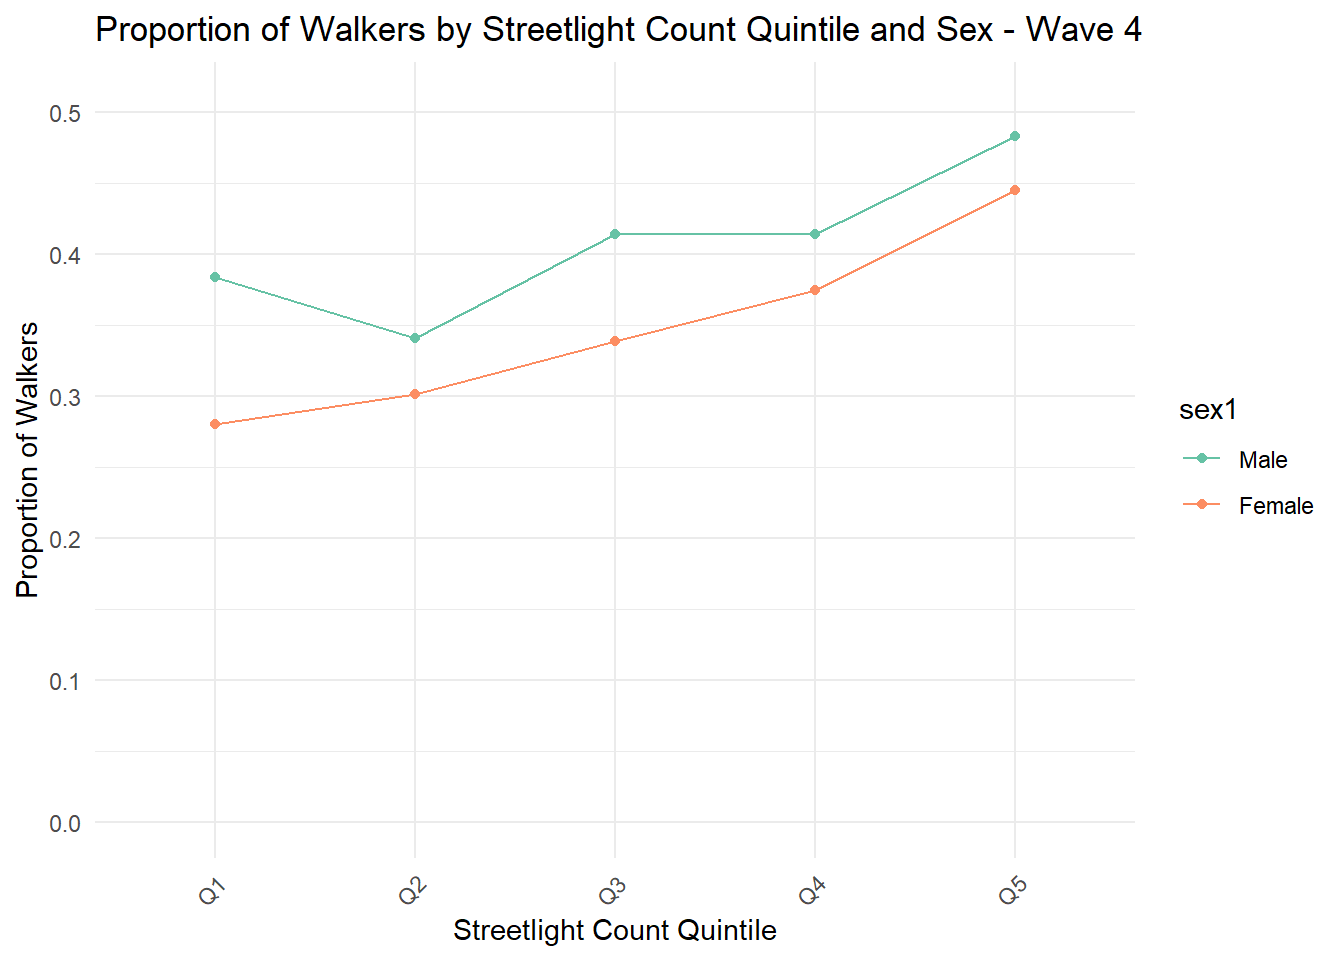
\includegraphics{_main_files/figure-latex/walkers.Prop_vs_SL_plot-4.pdf} 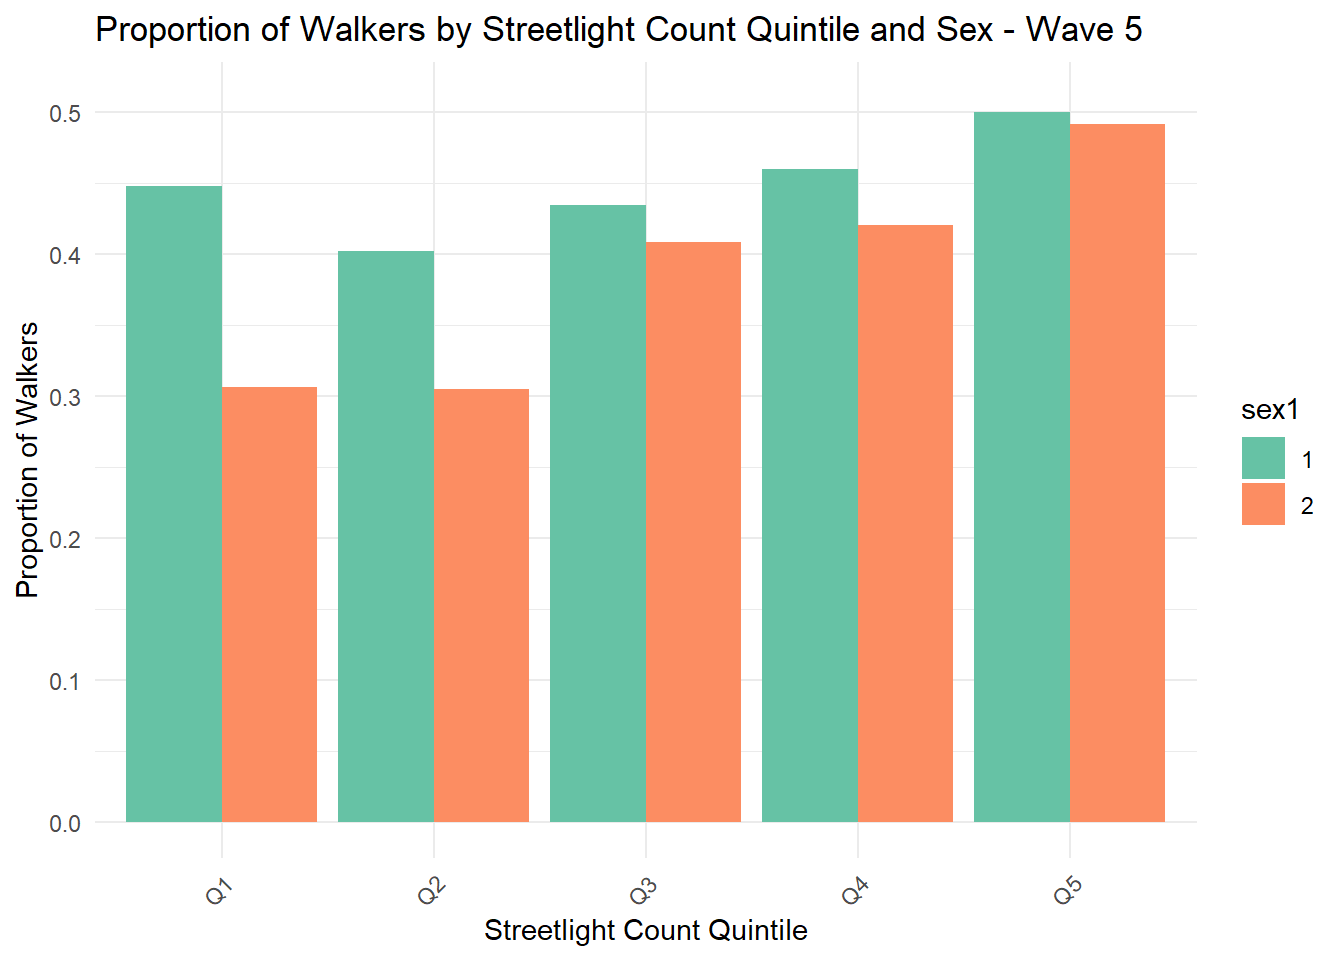
\includegraphics{_main_files/figure-latex/walkers.Prop_vs_SL_plot-5.pdf}

  \bibliography{book.bib,packages.bib}

\end{document}
